\section{DevOps}
\label{sec:devops}

\subsection{Build Automation}

\subsubsection{Gradle as a multi-language orchestrator}

Gradle is the project's primary build system, set up as a single multi-project build. The root holds two files: \texttt{build.gradle.kts}, defining project-wide tasks (environment setup, Docker environment orchestration and git pre-commit helpers), and \texttt{settings.gradle}, which registers every subproject and configures the git hooks.

Each service is a Gradle subproject, but the build spans different languages. JVM/Scala services (\texttt{events}, \texttt{users}) build natively through Gradle, while JS/TS services (\texttt{chat}, \texttt{interactions}, \texttt{media}, \texttt{notifications}, \texttt{ticketing} and the \texttt{frontend}) are wrapped via the node-gradle plugin, which delegates the actual work to npm. A single Gradle invocation thus drives heterogeneous toolchains behind one uniform task interface.

The monorepo layout was preferred because it enables:
\begin{itemize}
  \item \textbf{unified build and CI}: one Gradle invocation builds, checks and tests the whole system, and a single CI pipeline validates every service;
  \item \textbf{frictionless code sharing}: the libraries under \texttt{libs/} are consumed directly by the Node services, with no external registry publishing;
  \item \textbf{single versioning} for the whole product;
  \item \textbf{simplicity for a small team}: one repository, one build and one set of conventions keep the maintenance and cognitive overhead low.
\end{itemize}

\subsubsection{Convention plugins and custom tasks}

To avoid duplicating build logic, \texttt{buildSrc/} defines two \textbf{convention plugins}, one for the Scala services and one for the JS/TS ones. Each encapsulates the language-specific compilation, style and coverage setup and exposes it under a common set of task names.

A custom \texttt{ExecTask} further simplifies running arbitrary shell commands, with sequential chaining, \texttt{onSuccess}/\texttt{onFailure} callbacks and built-in cross-platform support. Shared constants are also defined alongside it under \texttt{buildSrc/}.

\subsubsection{Git hooks}

Hooks are installed through the \href{https://plugins.gradle.org/plugin/org.danilopianini.gradle-pre-commit-git-hooks/2.1.5}{\texttt{gradle-pre-commit-git-hooks}} plugin configured in \texttt{settings.gradle}. Two \textbf{pre-commit} hooks are registered:
\begin{itemize}
  \item \textbf{\texttt{formatAndLintPreCommit}} runs the format-and-lint task (which every subproject configures via its convention plugin), then re-stages the files that were staged at commit time, so any style fix is included in the commit;
  \item \textbf{\texttt{updateAndCheckEnvSetup}} updates \texttt{.env} from \texttt{.env.template} (adding any missing variable) and verifies that both files share the same keys and that \texttt{.env} values are populated, so a variable added only to the local \texttt{.env} cannot be pushed without also being declared in the shared \texttt{.env.template}.
\end{itemize}

A \textbf{commit-msg} hook additionally validates the commit message against the Conventional Commits convention.

\subsection{Dockerization}

\subsubsection{Dockerfile design}

Every service ships its own \texttt{Dockerfile}, designed around two goals: \textbf{layer caching} and \textbf{minimal image size}. Instructions are ordered properly for maximising cache reuse, and each image uses a \textbf{two-stage build}: a builder stage compiles the artifact while the final stage carries only the runtime plus the built output.

\subsubsection{Docker Compose layer system}

Every service and infrastructure component defines its Compose files, which are not standalone: utility scripts (\texttt{findComposeFiles.sh}, \texttt{composeAll.sh}) discover them and \textbf{merge them in layers}, each adding a concern on top of the previous one:

\begin{itemize}
  \item \textbf{base} (\texttt{docker-compose-base.yml}) --- the canonical service definition: image, networks, environment and healthchecks;
  \item \textbf{main} (\texttt{docker-compose.yaml}) --- production-oriented overrides: restart policy, Traefik routing labels and \texttt{depends\_on} conditions;
  \item \textbf{dev} (\texttt{docker-compose-dev.yaml}) --- development extras: local image \texttt{build}, exposed host ports and dev tooling (e.g. mongo-express);
  \item \textbf{swarm} (\texttt{docker-compose-swarm.yaml}) --- Swarm-specific settings: \texttt{deploy} (replicas, placement constraints, restart policy), overlay networks and configs.
\end{itemize}

A standard deploy merges \texttt{base $\rightarrow$ main}; a development environment adds \texttt{dev} on top; a Swarm deploy (beta) merges \texttt{base $\rightarrow$ swarm} instead of the main file.

\subsection{DVCS}

\subsubsection{Git Flow}

The repository follows a Git-Flow-inspired strategy: a single long-lived branch, \texttt{main}, updated exclusively through a \textbf{pull request} from feature branches. The merge strategy depends on the PR: small changes whose individual history carries little value are \textbf{rebased} to keep the history linear, while larger feature branches are integrated with \textbf{merge commits}, preserving the branch topology.

\subsubsection{Branch protection}

\texttt{main} is protected by a set of rules:
\begin{itemize}
  \item changes must arrive through a pull request \textbf{reviewed and approved by at least one other team member};
  \item the required CI status checks must pass before merging;
  \item direct pushes to \texttt{main} are blocked; the only whitelisted identity is a dedicated \textbf{GitHub App}, whose token lets the release workflow push the generated CHANGELOG.
\end{itemize}

Pull requests to \texttt{main} also enable automatic \textbf{Copilot review}, which gives an immediate first-pass on every PR, flagging obvious bugs and smells before a human reviewer steps in.

\subsubsection{Environment and secrets}

The \texttt{.env.template} file is the authoritative schema for the environment. Configuration variables are given a default value, while API keys and passwords are left empty. The \texttt{checkEnvSetup} task leverages this convention to enforce two properties:
\begin{enumerate}
  \item it \textbf{fails on empty values}, forcing real secrets to be provided locally and removing the risk of shipping placeholder credentials;
  \item it \textbf{fails on key mismatches} between \texttt{.env} and \texttt{.env.template}, keeping the schema in sync.
\end{enumerate}

To still allow building and testing in CI the pipeline injects default passwords before the check runs. Variables and secrets actually needed by the workflows are stored as \textbf{GitHub Actions Variables/Secrets}.

\subsection{CI/CD Pipelines}

\subsubsection{Quality gates on pull requests}

Three workflows act as quality gates on every pull request to \texttt{main}:

\begin{itemize}
  \item \textbf{\texttt{build-and-test.yml}} runs \texttt{./gradlew clean build} across all services (compile, check and test) and uploads coverage reports to \textbf{Codecov}; on pull requests it additionally detects which \texttt{Dockerfiles} changed and builds those images, validating that they build cleanly before the code lands.
  \item \textbf{\texttt{check-style.yml}} runs \texttt{./gradlew checkStyle} to verify linting and formatting.
  \item \textbf{\texttt{check-commit-convention.yml}} inspects every commit in the PR and validates it against the Conventional Commits specification.
\end{itemize}

Style and commit-convention checks are also enforced as git hooks, but they are re-checked in CI because hooks can be bypassed locally.

\subsubsection{Translation check}

The \textbf{\texttt{auto-i18n.yml}} workflow runs the project's own \texttt{auto-i18n} action on pushes to the frontend feature branch (\texttt{feature/frontend-service}) and on every pull request. On push it generates the missing translations and commits them; on pull requests it runs in \textbf{check-only} mode. To avoid re-triggering the pipeline on the auto-generated commit, the commit message carries \texttt{[skip ci]}, which is omitted when a PR is already open from that branch, so that all required checks still run.

\subsubsection{GitHub Pages}

The \textbf{\texttt{deploy-pages.yml}} workflow triggers on pushes to \texttt{main} and to any \texttt{docs/*} branch. It builds the three VitePress report sites (ASW, DS, SPE), copies the static assets and the OpenAPI/AsyncAPI specifications into the output tree, and publishes everything to \textbf{GitHub Pages}.

\subsubsection{Release and Deploy}

Every push to \texttt{main} triggers the \texttt{release.yml} pipeline, which first decides whether a release is needed:
\begin{itemize}
  \item \textbf{semantic-release} inspects the commits and publishes a new versioned release following Conventional Commits + SemVer;
  \item if no release is published but \texttt{services/} or \texttt{infrastructure/} changed, the pipeline falls back to an incremental \textbf{dev pre-release} (e.g. \texttt{v1.4.0-dev.2}), so that every meaningful change still produces a deployable tag.
\end{itemize}

When a tag is produced, the pipeline finds all modified directories containing a \texttt{Dockerfile}, then builds and pushes the corresponding \textbf{multi-arch images} (\texttt{linux/amd64} + \texttt{linux/arm64}, via Buildx and QEMU) to \texttt{ghcr.io}. The service name is derived from the Dockerfile path (e.g. \texttt{services/chat/Dockerfile} $\rightarrow$ \texttt{chat}). Each image is pushed under two tags: the \textbf{release version} (e.g. \texttt{chat:2.2.2}) and \textbf{\texttt{:latest}}.

The deployed production infrastructure is the following:

\begin{figure}[H]
  \centering
  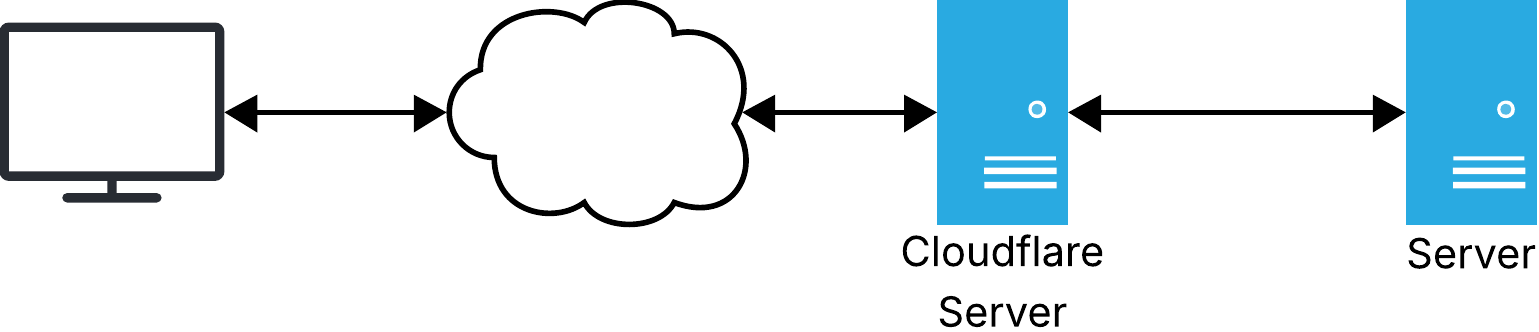
\includegraphics[width=\textwidth]{../public/devops/deployed-infrastructure.png}
  \caption{Deployed infrastructure}
\end{figure}

The deploy job then opens an SSH session to the production server through a \textbf{Cloudflare Tunnel}: the connection is authenticated via Cloudflare Access and bridged through Cloudflare's network, so no SSH port is exposed publicly. On the remote machine the repository is pulled, the new images are pulled from the registry and the stack is redeployed via \texttt{composeApplication.sh}.

A \textbf{Docker Swarm} deployment path is also available (still in beta): \texttt{scripts/swarmDeploy.sh} manages the full Swarm lifecycle, including pushing the images to Docker Hub so they are reachable from every swarm node.
